\documentclass[border=8pt]{standalone}
\usepackage{fontspec}
\defaultfontfeatures{Ligatures=TeX}
\setmainfont{Palatino Linotype}
\setsansfont{Arial}
\usepackage{amsmath,amssymb}
\usepackage{tikz}
\usetikzlibrary{arrows.meta,positioning,calc,shapes.geometric,fit}
\definecolor{tksInk}{HTML}{1C1A16}
\definecolor{tksMuted}{HTML}{8A8378}
\definecolor{tksAccent}{HTML}{8C5A1F}
\definecolor{tksAfill}{HTML}{F6EEDD}
\definecolor{tksAedge}{HTML}{9A7328}
\definecolor{tksBfill}{HTML}{E6EDF5}
\definecolor{tksBedge}{HTML}{2F5B85}
\definecolor{tksCfill}{HTML}{F7E7E4}
\definecolor{tksCedge}{HTML}{95403A}
\definecolor{tksDfill}{HTML}{E4EFE6}
\definecolor{tksDedge}{HTML}{3A6B45}
\definecolor{tksEfill}{HTML}{F5DFDC}
\definecolor{tksEedge}{HTML}{A33B30}
\begin{document}
\centering
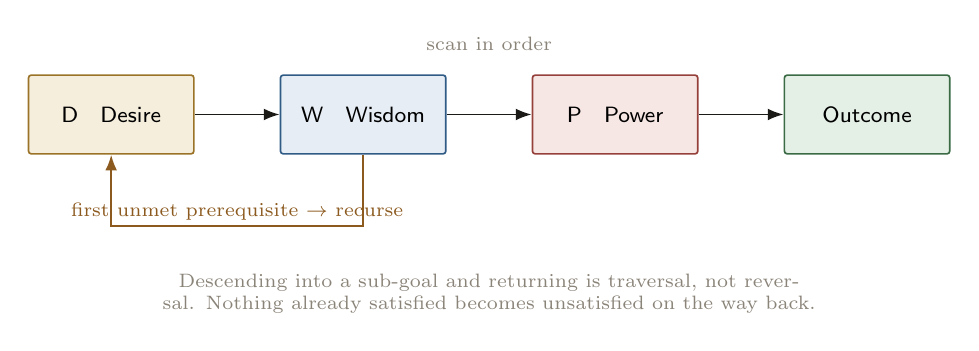
\begin{tikzpicture}[x=1mm, y=1mm, font=\sffamily\footnotesize,
  st/.style={rounded corners=1pt, minimum width=21mm, minimum height=10mm,
             draw, line width=0.6pt}]
  \node[st, fill=tksAfill, draw=tksAedge] (D) at (0,0)   {D \; Desire};
  \node[st, fill=tksBfill, draw=tksBedge] (W) at (32,0)  {W \; Wisdom};
  \node[st, fill=tksCfill, draw=tksCedge] (P) at (64,0)  {P \; Power};
  \node[st, fill=tksDfill, draw=tksDedge] (O) at (96,0)  {Outcome};
  \foreach \a/\b in {D/W, W/P, P/O} {
    \draw[-{Latex[length=2mm]}, tksInk, line width=0.7pt] (\a) -- (\b);
  }
  \node[font=\scriptsize, text=tksMuted] at (48,9) {scan in order};
  % recursion on the first unmet prerequisite
  \draw[-{Latex[length=2mm]}, tksAccent, line width=0.7pt]
    (W.south) -- ++(0,-9) -- ++(-32,0) -- ++(0,9);
  \node[anchor=north, font=\scriptsize, text=tksAccent] at (16,-10)
    {first unmet prerequisite $\rightarrow$ recurse};
  \node[anchor=north, text width=92mm, align=center, font=\scriptsize,
        text=tksMuted] at (48,-19)
    {Descending into a sub-goal and returning is traversal, not reversal.
     Nothing already satisfied becomes unsatisfied on the way back.};
\end{tikzpicture}
\end{document}
